%**********************************************************
\subsection{Task Overview}
One can define and describe briefly how the local system is implemented, making use of threads and processes. As one can see in figure \ref{fig:task_overview}, this system is composed by two processes: the main process and a daemon, used to read all the sensors, \textit{dSensors}. The communication between the daemon and the main process is done via pipe.

\begin{figure}[H]
	\centering
	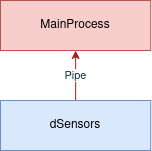
\includegraphics[width=.3\textwidth]{09sw_specification/task_overview}
	\caption{Inter-process Communication between Main Process and Daemon.}
	\label{fig:task_overview}
\end{figure}

One can list the tasks that compose the main process:
\begin{itemize}
	\item \textbf{tCamera:} acquire a camera frame; processes image and search for parking spots; verify the parking spot availability;
%	\item \textbf{tLampControl:} initializes PWM interface; controls the PWM applied to the lamp;
	\item \textbf{tLoraSend:} sends a message to the gateway, using the LoRa module;
	\item \textbf{tLoraRecv:} receives a message from the gateway, using the LoRa module;
	\item \textbf{tRecvSensor:} receives messages sent by the daemon, via pipe, regarding sensors information.
\end{itemize}

%**********************************************************
\subsection{Task Priority}

%**********************************************************
\subsection{Task Synchronization}
Real-time tasks share resources and services, and as such, should be prepared to await for the availability of these resources and services, like logical resources (buffers and data), physical resources, services like directory services, etc. In order to have coordinate access to shared resources and avoid race conditions, the kernel has resources that provide synchronization tools. 

\myparagraph{Condition Variables}

A condition variable is a task synchronization tool that can be used to block (wait) one or more threads, suspending its execution. The blocked threads are awakened when the condition variable is notified. The condition variables used are listed below.

\begin{itemize}
	\item \textbf{condCameraAcquire:} used to notify \textit{tCamera} that a camera sample period has elapsed;
	
%	\item \textbf{condNewPWM:} used to notify \textit{tLampControl} that a new PWM value for the lamp was defined;
	
	\item \textbf{condSend:} used to notify \textit{tLoraSend} that a new message is ready to be sent;
	
	
\end{itemize}

\myparagraph{Mutexes}
A mutex is a locking mechanism that provides mutual exclusion, supporting ownership and other protocols. A mutex is initially created in the unlocked state in which it can be acquired by a task. After being acquired, the mutex moves to the locked state. When the task releases the mutex, it returns to the unlocked state. The mutexes used are listed bellow.

\begin{itemize}
	\item \textbf{mutCamera:} mutex associated with the condition variable \textit{condCameraAcquire} to acquire a camera frame;
		
	\item \textbf{mutSend:} protects the message to be sent in \textit{tLoraSend}, which can be defined in multiple places;
	
	\item \textbf{mutComms:} protects LoRa communication, since it is half-duplex, so one can send or receive at a time; Used in \textit{tLoraSend} and \textit{tLoraRecv};
	
	\item \textbf{mutChangePWM:} protects the modification of PWM when defining a new PWM value for the lamp;
	
	
\end{itemize}

%\myparagraph{Semaphores}

\subsection{Task Communication}
\myparagraph{Pipes}
Pipe is an inter-process communication tool, that establishes a connection between two processes, such that the standard output from one process becomes the standard input of the other process. Pipe is one-way communication, i.e, we can use a pipe such that one process write to the pipe and the other process reads from the pipe. If a process tries to read before something is written to the pipe, the process is suspended until something is written.

As previously stated, it's used a pipe to communicate between the \textit{dSensors} to the main process. In this way, the main process can know if something was detected by the sensors and provide a response to that.

%\myparagraph{Signals}

%**********************************************************
\subsection{Class Diagrams}
\myparagraph{Class Camera}

\myparagraph{Class Lamp}

\myparagraph{Class Communications}

%**********************************************************
\subsection{Flowcharts}
\clearpage
\myparagraph{tCamera}

The task tCamera is responsible for acquire a frame from the Raspberry Pi Camera and to process it. It must analyze the returned frame, in order to detect empty parking spots. This thread uses the mutex \textit{mutCamera} to protect the condition variable \textit{condCameraAcquire}, that synchronizes the camera frame acquisition with the timer that defines the camera frame acquisition period, \textit{timSampleCam}.

Firstly, this thread initializes the camera device, sets the timer \textit{timSampleCam}, locks the mutex \textit{mutCamera} and goes to sleep mode, waiting for the conditon variable \textit{condCameraAcquire} to be signaled. This happens when a \textit{timSampleCam} period has elapsed and the thread wakes up. Now, one can read a camera frame in order to process it, unlocking the mutex \textit{mutCamera}. A timer, \textit{timCamMax}, is setted to report the error if the image is taking too much time to being processed.

In the image processing part of the thread, if there aren't parking spots coordinates stored, then it is necessary to search for parking spots. After that, one can detect cars using the pre-trained model and the function \textit{detectMultiScale} that detects objects in the image. If the coordinates of a detected car matches the coordinates of the parking spot, then one can assume that the parking spot is occupied. If the parking spot status has changed, then it is necessary to send this to the remote system, using the LoRa communication module.

\myparagraph{tLampControl}
% uses: mutChangePWM; condNewPWM; pwm_val
% pwm_val is used in: PIR_sensor, CommandCb, LDR
% must define: MIN_BRIGHT_PWM; LAMP_ON_TIMEOUT
This task is responsible for initializing and controlling the PWM peripheral used to control the lamp brightness. A mutex \textit{mutChangePWM} is used to protect the process of defining a new PWM value. 

After initializing the PWM, this task goes to sleep, waiting for the condition variable \textit{condNewPWM} to notify this task. This happens when a new PWM value is defined into the variable \textit{pwm\_val}, in \textit{dReadSensors} or in a received command. Then, the lamp PWM is changed to the new value. 

The lamp may have various levels of luminosity: for the lamp to be OFF, is applied PWM~=~0; for the lamp to be at a predefined minimum bright level, is applied PWM~=~\textit{MIN\_BRIGHT\_PWM}; for the lamp to be at maximum bright, this is, when the lamp must be ON, is applied PWM~=~100. So, since the lamp must stay ON a minimum amount of time out of a motion is detected or out of a request from the remote system to be ON, one needs to check if the new PWM is the maximum value. If so, that means that the lamp should continue with that PWM for a predefined time, defined by \textit{LAMP\_ON\_TIMEOUT}, in seconds.

\myparagraph{tLoraSend}

\myparagraph{tLoraRecv}

% FLOWCHARTS SENSORS

\myparagraph{PirIsr}
The PIR sensor uses the GPIO of the Raspberry Pi in order to inform the system if there's movement in the surrounding area. In the afirmative case, it puts the high digital value on its output, and this can be used to generate an interrupt service routine, triggered on the rising edge of the output signal of the sensor. When this routine is executed, it locks the mutex \textit{mutChangePWM} and assign the \textit{PWM\_val} its maximum value, 100 \%. This operation is signaled to the process that controls the lamp brightness through a pipe, and the mutex is unlocked. In the figure \ref{fig:pir_isr}, is represented the flowchart of the PirIsr function.

\begin{figure}[H]
	\centering
	%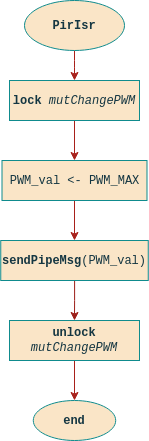
\includegraphics[width=.5\textwidth]{09sw_specification/pir_isr}
	\caption{PirIsr flowchart.}
	\label{fig:pir_isr}
\end{figure}

\myparagraph{LdrIsr}
The ambient light sensor, LDR, is used to determine when is time to turn on the lights, that is, when is night time and interfaces with the Raspberry Pi through I2C protocol communication. As the sun set or the sun rise is a relatively long time process, there's no need to keep checking the sensor output value all the time, so one can define a period to get the sensor value, \textit{LDR\_TIM}, that can be 10 minutes. In figure \ref{fig:ldr_isr} is shown the LDR sensor interrupt service routine, triggered by the timer overflow. When the timer period elapses, one can get the illuminance value calculated by the sensor. If this value is lower than the threshold value defined as good luminosity illuminance, GOOD\_LIGHT\_LUX, then the auxiliary variable, \textit{lowLightCon} is setted to high. In the next step, if the \textit{lightCon} variable (stores the last ambient light condition) is not equal to the auxiliary variable, then it is needed to change the \textit{lightCon} variable and send de pipe message to the process that controls the lamp PWM. 

\begin{figure}[H]
	\centering
	%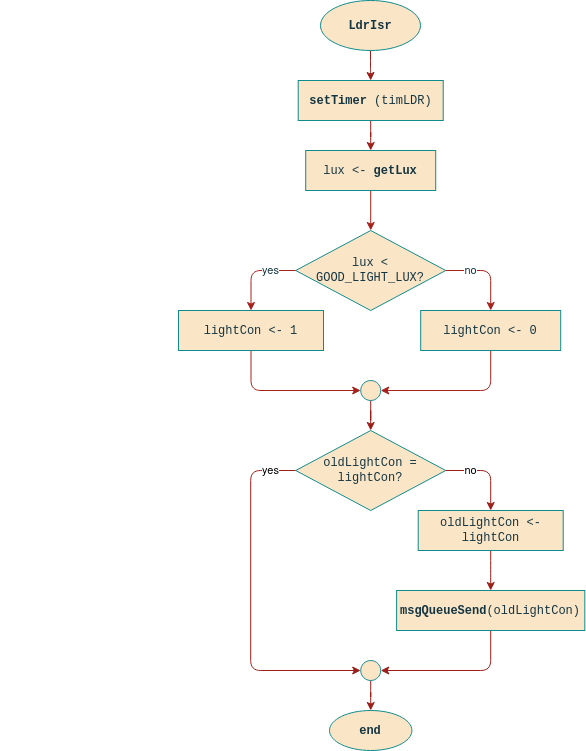
\includegraphics[width=.5\textwidth]{09sw_specification/ldr_isr}
	\caption{LdrIsr flowchart.}
	\label{fig:ldr_isr}
\end{figure}

\myparagraph{FailureDetectIsr}
In figure \ref{fig:fail_isr} is represented the FailureDetectIsr flowchart. Similarly to the PIR sensor, this routine is triggered on the rising edge of the output signal of the sensor. When the Failure detector detects that the lamp is broken, it puts the high digital value in its output, triggering this function. In this routine, the PWM is setted to 0 \% and are sent two messages through pipes: one to inform the process, that controls the lamp, to change the PWM value in the channel; and the other to notify the remote system that the lamp is broken, in order to update this status on the database.

\begin{figure}[H]
	\centering
	%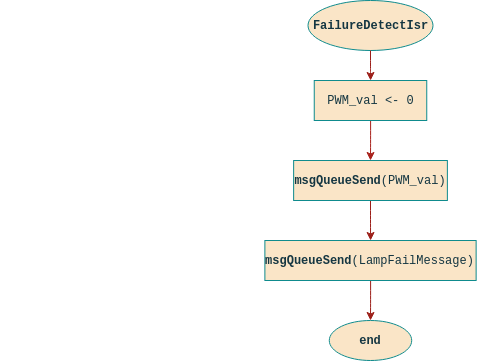
\includegraphics[width=.5\textwidth]{09sw_specification/fail_isr}
	\caption{FailureDetectIsr flowchart.}
	\label{fig:fail_isr}
\end{figure}

%**********************************************************
\subsection{Start-up Process}

%**********************************************************
\subsection{Shutdown Process}

